\documentclass[10.7pt,]{article}

\usepackage[letterpaper, margin=2.54cm, top=2.54cm]{geometry}
\usepackage[super,comma,sort&compress]{natbib}
\usepackage{lmodern}
\usepackage{authblk} % To add affiliations to authors
\usepackage{amssymb,amsmath}
\usepackage{wrapfig}
\usepackage{graphicx,grffile}
\usepackage[labelfont=bf,labelsep=period]{caption}
\usepackage{ifxetex,ifluatex}
\usepackage{bm}
\usepackage{array, boldline, makecell, booktabs}
\usepackage{multirow}


%\usepackage{fixltx2e} % provides \textsubscript
\ifnum 0\ifxetex 1\fi\ifluatex 1\fi=0 % if pdftex
  \usepackage[T1]{fontenc}
  \usepackage[utf8]{inputenc}
\else % if luatex or xelatex
  \ifxetex
    \usepackage{mathspec}
  \else
    \usepackage{fontspec}
  \fi
  \defaultfontfeatures{Ligatures=TeX,Scale=MatchLowercase}
    \setmainfont[]{Arial Narrow}
    \setsansfont[]{Century Gothic}
    \setmonofont[Mapping=tex-ansi]{Consolas}
\fi
% use upquote if available, for straight quotes in verbatim environments
\IfFileExists{upquote.sty}{\usepackage{upquote}}{}
% use microtype if available
\IfFileExists{microtype.sty}{%
	\usepackage{microtype}
	\UseMicrotypeSet[protrusion]{basicmath} % disable protrusion for tt fonts
}{}

\usepackage{lipsum} % for dummy text only REMOVE

\newtheorem{exm}{Example}


%==============================
% Customization to make the output PDF 
% look similar to the MS Word version
%==============================
% To prevent hyphenation
\hyphenpenalty=10000
\exhyphenpenalty=10000

% To set the sections font size
\usepackage{sectsty}
\allsectionsfont{\fontsize{11}{11}\selectfont}
\sectionfont{\fontsize{14}{14}\selectfont}
\subsectionfont{\bfseries\fontsize{13}{13}\selectfont}
\subsubsectionfont{\bfseries\fontsize{11}{11}\selectfont}
%\subsubsectionfont{\normalfont}

% Spacing
\usepackage{setspace}

\usepackage{xcolor}

% No new line after subsubsection
\makeatletter
%\renewcommand\subsubsection{\@startsection{subsubsection}{3}{\z@}%
%	{-3.25ex\@plus -1ex \@minus -.2ex}%
%    {-1.5ex \@plus -.2ex}% Formerly 1.5ex \@plus .2ex
%    {\normalfont}}
%\makeatother

\makeatletter % Reference list option change
\renewcommand\@biblabel[1]{#1.} % from [1] to 1
\makeatother %

% To set the doc title font
\usepackage{etoolbox}
\makeatletter
\patchcmd{\@maketitle}{\LARGE}{\bfseries\fontsize{15}{16}\selectfont}{}{}
\makeatother

% No page numbering
\pagenumbering{gobble}

\makeatletter
\def\maxwidth{\ifdim\Gin@nat@width>\linewidth\linewidth\else\Gin@nat@width\fi}
\def\maxheight{\ifdim\Gin@nat@height>\textheight\textheight\else\Gin@nat@height\fi}
\makeatother

% Scale images if necessary, so that they will not overflow the page
% margins by default, and it is still possible to overwrite the defaults
% using explicit options in \includegraphics[width, height, ...]{}
\setkeys{Gin}{width=\maxwidth,height=\maxheight,keepaspectratio}
\setlength{\parindent}{0pt}
\setlength{\parskip}{6pt plus 2pt minus 1pt}
\setlength{\emergencystretch}{3em}  % prevent overfull lines
\providecommand{\tightlist}{%
  \setlength{\itemsep}{0pt}\setlength{\parskip}{0pt}}
\setcounter{secnumdepth}{0}
% Redefines (sub)paragraphs to behave more like sections
\ifx\paragraph\undefined\else
\let\oldparagraph\paragraph
\renewcommand{\paragraph}[1]{\oldparagraph{#1}\mbox{}}
\fi
\ifx\subparagraph\undefined\else
\let\oldsubparagraph\subparagraph
\renewcommand{\subparagraph}[1]{\oldsubparagraph{#1}\mbox{}}
\fi
%==============================
\usepackage{hyperref}
\hypersetup{
	unicode=true,
	pdftitle={My Cool Title Here},
	pdfauthor={Author One, Author Two, Author Three},
	pdfkeywords={keyword1, keyword2},
	pdfborder={0 0 0},
	breaklinks=true
}
\urlstyle{same}  % don't use monospace font for urls

% Keywords command
\providecommand{\keywords}[1]
{
  \small	
  \textbf{Key words---} #1
}
%==============================

% reduce space between title and begining of page
\title{\vspace{-2em} Not So Weak-PICO: Leveraging weak supervision for Participants, Interventions, and Outcomes extraction for systematic review automation}
\date{\vspace{-5ex}}
\author[ ] {
    % Authors
    \bf\fontsize{13}{14}\selectfont
    Anjani Dhrangadhariya,\textsuperscript{\rm 1, 2}
    Henning M\"uller \textsuperscript{\rm 1, 2}
}
\affil[1]{Institute of Business Information Systems, University of Applied Sciences Western Switzerland (HES-SO Valais-Wallis), Sierre, Switzerland}
\affil[2]{Department of Computer Science, University of Geneva (UNIGE), Geneva, Switzerland}
\affil[*]{Corresponding author: Anjani Dhrangadhariya, Institute of Business Information Systems, University of Applied Sciences Western Switzerland (HES-SO Valais-Wallis), Sierre, Switzerland; anjani.dhrangadhariya@hevs.ch}
%==============================
\begin{document}
\maketitle
\vspace{2em} %separation between the affiliations and abstract
%==============================
\doublespacing
%==============================
\section{ABSTRACT}
\label{abstract}
%==============================
% Note: Abstract is limited to 250 words
%
\textbf{Objective:}
PICO analysis is a vital but time-consuming task for conducting systematic reviews (SR). 
Supervised machine learning methods can help fully automate PICO analysis, but a lack of large annotated corpora restricts innovation and adoption of automated PICO recognition systems.
The largest-available PICO entity corpus is manually annotated, which is too expensive for the most scientific community.
Additionally, depending upon the SR question, PICO criteria are extended to PICOS (S-Study type or design), PICOC (C-Context), and PICOT (T-timeframe) meaning the static hand-labelled corpora should undergo costly re-annotation as per the downstream requirements.
We test feasibility of developing a weak supervision system to extract PICO without hand-labelled data.\\
\textbf{Materials and Methods:}
We investigate a weak supervision approach using medical ontologies and expert-generated rules for PICO entity recognition without relying on hand-labelled data.
\textbf{Results:}
We present Weak-PICO+, a method for weakly supervised PICO entity recognition using medical ontologies, non-medical ontologies and expert-generated rules.
Unlike manual annotation, Weak-PICO+ does not use any hand-labelled data and is quickly adaptable and extensible to other entities.
We demonstrate this through extracting an additional Study Type and Design entity making PICO go PICOS without manual annotation effort.\\
\textbf{Conclusion:}
Weak supervision using weak-PICO+ for PICO entity recognition has good results and extends to more clinical entities without hand-labelled data.\\
%
%
%


\keywords{Randomized Controlled Trials, Weakly-Supervised Machine Learning, Information Extraction, Evidence-based Medicine}
%
\clearpage
% Full paper is limited to 4000 words (approx. 14.6 pages)
%
%
%
%==============================
\section{INTRODUCTION}\label{introduction}
%==============================
%
Systematic Review (SR) is an evidence-based practice of answering clinical questions using a transparent and quantitative approach whereby the reviewers must collect as many research publications as possible, identifying the relevant publications from these and integrating their results via statistical analysis.
Filtering relevant publications from the bulk collected ones often uses PICO (Participants, Interventions, Comparators, Outcomes) criteria. 
A clinical study or a publication is relevant only for answering a question only if it studies question relevant participants, interventions (and their comparators) and outcomes. 
Manually analysing PICO information from thousands of publications for a single SR takes about 12 months of two medical experts' time.
The process can be automated using machine learning based information extraction strategies by directly pointing the human reviewers to the correct text chunks describing PICO.
Machine learning classifiers rely on hand-labelled training corpora.
Hand labelling corpora with PICO information for a downstream IE application requires people with combined medical and informatics skills, is expensive and time-consuming in terms of the actual annotation process and annotator training.


Extracting PICO information is somewhat tricky because of high disagreement between human annotators on the exact spans constituting PICO.
This leads to human errors in hand-labeled corpora.
Additionally, depending upon the systematic review question, PICO criteria are extended to PICOS (S-Study design), PICOC (C-Context), and PICOT (T-timeframe).
Hand-labeled datasets are static and prohibit quick manual re-labeling in case of human errors or when a downstream task requires new entities.
Additionally, in SRs, the step after PICO information analysis is to identify risk of bias from the studies which is another information extraction lacking a manually labelled corpora. 
This annotation bottleneck across domains has shifted gears in favour of weakly-supervised learning that relies on programmatic labelling sources to obtain training data.
Programmatic labelling is quick and allows efficient modifications to the training data labels as per the downstream application changes.


Medical ontology compendium like UMLS with several vocabularies, other external vocabularies and open access knowledgebases are an excellent resource for building clinical entity labelled training data~\cite{humphreys1998unified}. 
Legacy clinical applications both in NLP and image analysis are often automated using a multiple \textit{if-else} rules relying on key-phrases and visual cues (refer to document and image classification methods that are rule based).
The bottleneck here is how to combine these labelling sources of varying accuracy and strength.
Combining multiple labeling sources of variable accuracy is one of challenges.
%\textcolor{blue}{Give some paper examples where they utilize non-generative models to combine multiple labelling sources.}
There have been some fundamental works investigating how to combine multiple label sources of variable accuracy by ranking their importance based on their probability of error and efficiently assembling them.
The problem of aggregating several weak labellers have now transitioned to training a generative model that estimates the accuracy of each labelling source~\cite{ratner2016data,safranchik2020weakly,lison2021skweak}.
\textcolor{blue}{Expound on weakly-supervised learning and generative modelling using Snorkel, AutoNER, Swellshark.}



Weakly-supervised learning has demonstrated its prowess for clinical document classification and relation extraction, but clinical entity extraction tasks have relied on fully-supervised approaches.
relation extraction (Distant supervision for relation extraction without labeled data, Distant supervision for relation extraction without labeled data)
document classification (Weakly-Supervised Neural Text Classification
, Leveraging Large Amounts of Weakly Supervised Data for
Multi-Language Sentiment Classification)
\textcolor{blue}{Give examples of weakly supervised learning approaches for document classification and relation extraction.}
Combining multiple weak labeling sources for clinical entity extraction have been explored by Fries et al. in their paper Trove.
Trove uses Snorkel which is a generative model implemented in python and is a domain agnostic methodology to combine multiple labelling sources of variable accuracy.
However, Trove only explores the very defined entities like chemical, disease, disorder and drug classes. 
By definition, PICO information are spans that encompass multiple sub-class entities.
A shortcoming of span extraction is that even after a machine points a human reviewer to the correct PICO span, the reviewer requires to manually read and understand its finer aspects to screen the study for relevance.
Span extraction hence leads to semi-automation but hinders full-automation.
Weakly-supervised PICO entity extraction has not garnered enough attention as much as supervised PICO span extraction.
As far as our knowledge goes, only two studies exist for weakly-supervised PICO extraction.
One of these approaches only explores weak supervision for intervention extraction using a single labelling source~\cite{dhrangadhariya2022distant}, and the other approach relies on a single source of programmatic labelling and focuses on PICO spans and sentences rather than entities.
Entity recognition approach to PICO is not as easy as entity recognition approach to disease or chemical names which are more or less standardised.
PICO terms are not standard and even the experts do not agree on the exact tokens constituting PICO~\cite{brockmeier2019improving}.

A Trove-like weak-supervision for PICO entities has several challenges.
Consideration 1: Defining the sub-classes or entities encompassed within PICO spans
Consideration 2: Mapping the several ontologies, vocabularies and terminologies to the target sub-classes of PICO.
Consideration 3: Developing weakly-supervised classifiers optimally combining several ontologies and evaluate its performance in comparison to fully-supervised approach.
Consideration 4: Extending the ontology-based classifiers using expert-generated rules and evaluate performance in comparison to fully-supervised approach. This serves as an ablation study whereby the importance of low cost ontology labellers could be compared to addition of high cost expert generated rules.
Consideration 5: Identifying lags in the currently available PICO training dataset and correcting it.

In this work, we demonstrate the feasibility of weakly-supervised PICO entity extraction using two benchmark test sets.
We show how using only ontology dependent classifiers vs combining them with more expensive expert-generated rules compares to fully-supervised PICO entity extraction.
%
%
%
%==============================
\section{METHODOLOGY}\label{methods}
%==============================
%
The birds-eye view of our approach is shown in the Figure.

\begin{figure}[t]
\centering
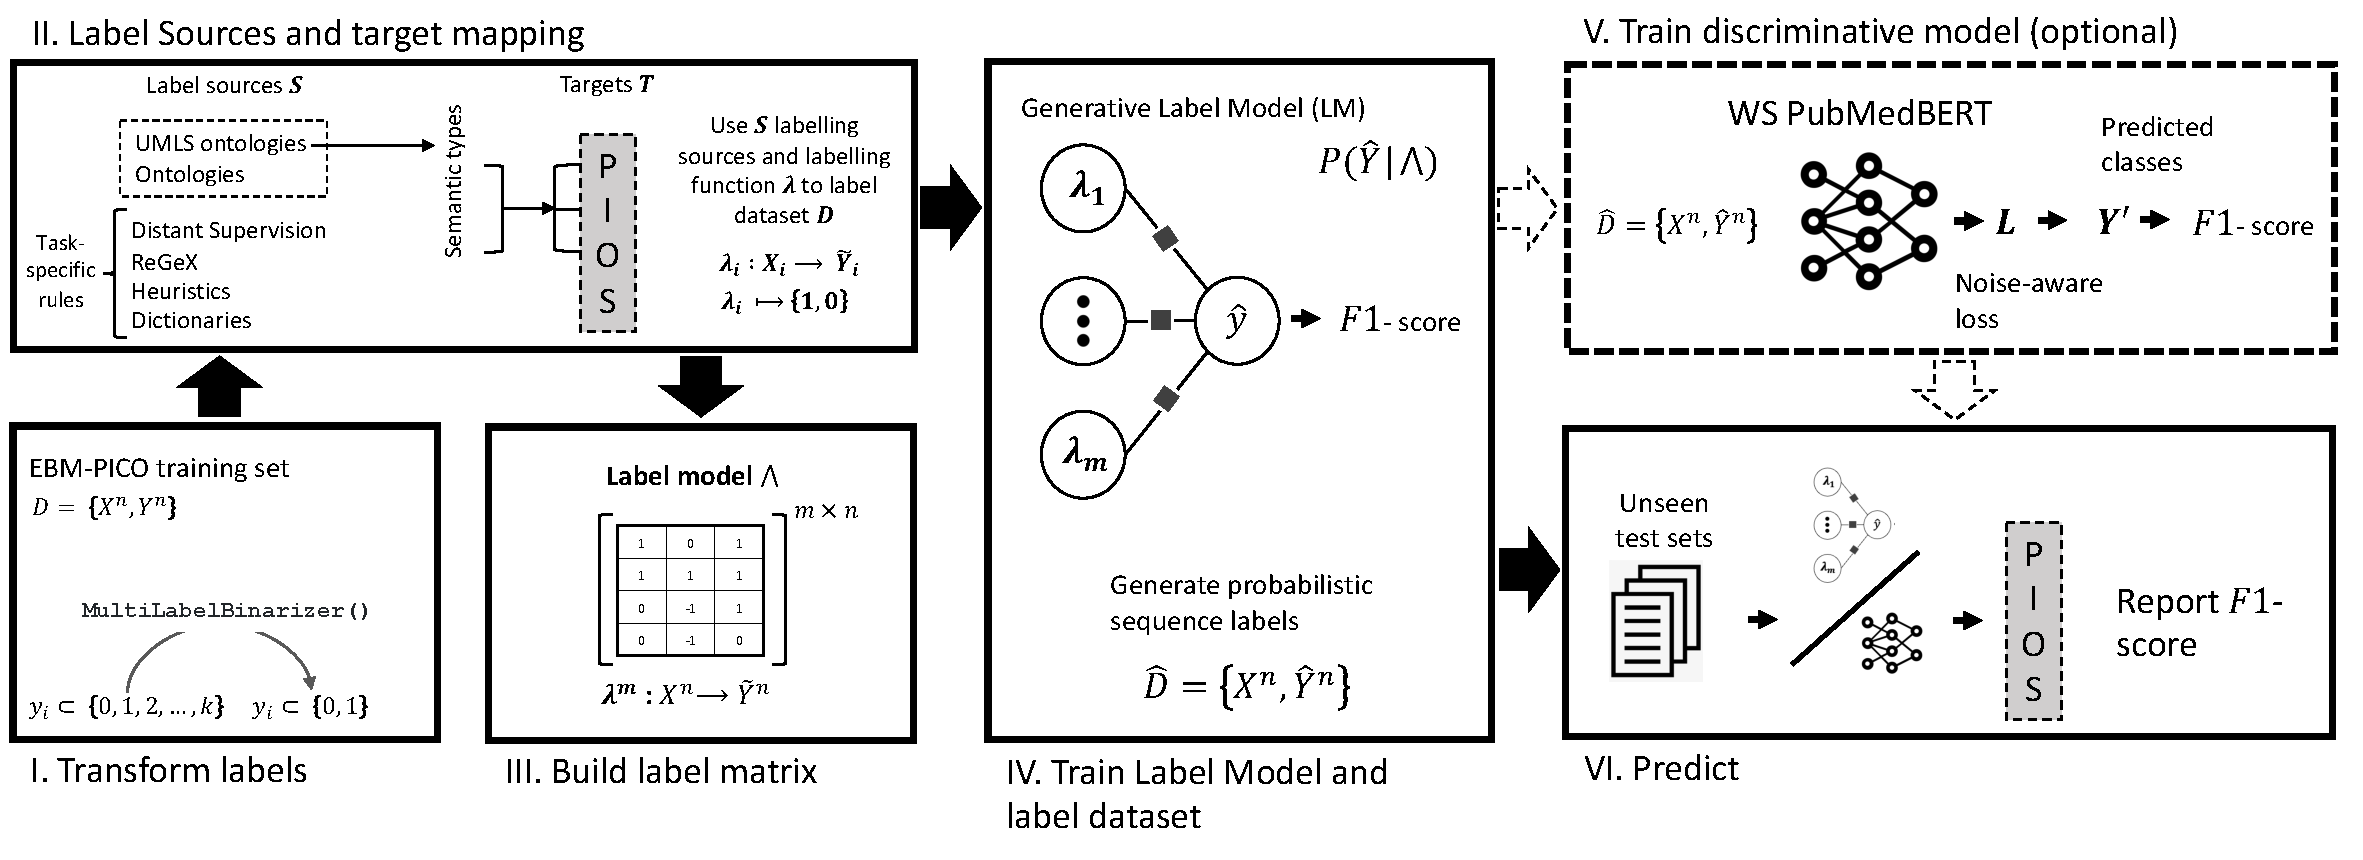
\includegraphics[width=0.98\textwidth]{figures/approach.pdf}
\caption{Approach overview.}
\label{fig:approach}
\end{figure}
%
%
%
%==============================
\subsection{Datasets and tasks}\label{data}
%==============================
%
\textbf{EBM-PICO.}
The EBM-PICO dataset is a widely used NLP benchmark with 5000 PICO annotated documents.~\footnote{A single document consists of a title and an abstract.}
The dataset has annotations at two levels: span-level or coarse-grained and entity-level or fine-grained (see Table~\ref{table:coarsefineconcept}).
Span level annotation encompasses the maximum information about each PICO class.
Entity-level PICO annotation covers fine-grained PICO information at the entity level, with PICO classes further divided into fine-grained subclasses.
The dataset comes pre-divided into a training set (n=4,933) annotated through crowd-sourcing and an expert annotated gold test set (n=191) for evaluation purposes.


\textbf{EBM-PICO corrected + Study type}
The EBM-PICO annotation guidelines caution about variable annotation quality~\footnote{https://www.ncbi.nlm.nih.gov/pmc/articles/PMC6174533/bin/NIHMS988059-supplement-Appendix.pdf}.
Variable annotation quality in the training dataset is pardonable, but the possible errors in the gold standard test set will impact the development of downstream extraction models.
The entity-level annotations in the EBM-PICO gold test set (n=191) have several errors that could lead to faulty evaluation of machine learning methods.
We evaluate 1\% of the EBM-PICO training set tokens to gauge the possible reasons for the errors.
We use this error evaluation exercise to conduct an error-focused corpus re-annotation for the EBM-PICO gold corpus (n = 191) for PICO entities.
 
We annotated an additional entity for study type only for this corpus to measure the effectiveness of weak supervision approaches.
Our study type entity is restricted to type and design (placebo-controlled, allocation, masking, intervention model) of a clinical study.
This annotation exercise was to demonstrate the application of weak supervision for entities beyond PICO~\cite{menard2019turning}.

\textbf{Physio set.} A test set comprising 153 PICO annotated documents from Physiotherapy and Rehabilitation RCTs (Randomized Controlled Trials) was used as an additional benchmark to evaluate the generalization power of our approach for this sub-domain~\cite{dhrangadhariya2021end}.

These datasets come tokenized, and we did not do additional preprocessing except adding complementary token information like POS tags, and token lemmas were obtained using spaCy.
Multi-class fine-grained PICO annotations were binarized i.e. a token label was set to 1 if the token represented an entity otherwise it was set to 0.
All the state of the art approaches use non-binarized labels for fine-grained PICO recognition making them incomparable to our approach.
%
%
%
\begin{table}[h!]
\begin{center}
\begin{tabular}{| c | c | c | c |} 
\hline
 & P & I/C & O \\ 
\hline
0 & No label & No label & No label \\ 
1 & Age & Surgical & Physical \\ 
2 & Sex & Physical & Pain \\
3 & Sample size & Drug & Mortality \\
4 & Condition & Educational & Side effect \\
5 &  & Psychological & Mental \\
6 &  & Other & Other \\
7 &  & Control &  \\
\hline
\end{tabular}
\caption{\label{table:coarsefineconcept} P (Participant), I (Intervention) and O (Outcome) represent the coarse-grained labels which are further divided into respective fine-grained labels.}
\end{center}
\end{table}
%
%
%
%==============================
\subsection{Sequence labeling}\label{seq_lab}
%==============================
%
Labelling a training set with PICO entities is a classical binary sequence labelling problem aiming to map input sequence of n text tokens, $ \bm{X} = (x_{1}, x_{2}, \dotso , x_{n} )$ to output sequence $\bm{Y} = (y_{1}, y_{2}, \dotso , y_{n} )$, where each $y_{i} \subset y$ is the label for token $x_{i}$.
In weak supervision, $\bm{Y}$ is unobserved, and the challenge is to devise and aggregate several conflicting low-accuracy labellers $\lambda^{m}$ labelling $\bm{X}$ and estimate $\bm{Y}$.
The estimates $\bm{\hat{Y}}$ of $\bm{Y}$ are assigned as probabilistic token labels of $\bm{X}$ leading to a weakly labelled dataset that can be used to train downstream ML models.


Coarse-grained PICO annotations in EBM-PICO are spans composed of multiple fine-grained subclasses.
For instance, the participant span can include information about different participant characteristics: disease, disorder, symptoms, age, gender, the sample size in clinical studies, ethnicity, language or geographical location.
The intervention span can include information about pharmaceutical drugs, chemicals, physical therapies, surgery, behavioural or educational therapies, and a placebo or active comparator.
Additional intervention information that could be marked is dosage, frequency and mode of administration.
The outcome spans can include the outcome names and how these outcomes were measured by having information about the scales, techniques and instruments used to measure them.
Our task was to design weak labellers $\lambda^{m}$ corresponding to this fine-grained information, efficiently aggregate them to get probabilistic class labels, use the weakly-labelled dataset for downstream PICO recognition tasks, correct the fine-grained PICO annotations errors in the EBM-PICO test set and evaluate the approach on both the EBM-PICO and its updated version.
%
%
%
%==============================
\subsection{Labelling sources}\label{lss}
%==============================
%
We used the 2021AB-full release of UMLS Metathesaurus English subset dump with 223 vocabularies. % Anjani: Give an overview of labelling sources in the introduction section.
After removing non-English and zoonotic source vocabularies as well as sources containing fewer than 500 terms, we remained with 131 vocabularies~\cite{humphreys1998unified}.
Terms in the selected vocabularies were preprocessed by removing stopwords, numbers, punctuation's and were lower-cased using Smart lower casing to preserve abbreviations.
Additional vocabularies included disease ontology (DO), Human Phenotype Ontology (HPO), Ontology of adverse events (OAE), Chemical entities of biological interest (ChEBI),  comparative toxicogenomics database (CTD) Chemical and Disease subclasses, Clinical Trials Ontology (NDD-CTO)~\cite{schriml2012disease,robinson2008human,he2014oae,de2010chemical,lin2021cto}.
Regular expressions (ReGeX) and heuristics like POS tag cues were used capture recurring class-specific patterns otherwise not captured by standardized terminologies. 
Our hand-coded dictionaries were for participant gender, participant disease abbreviation, generic intervention comparator terms, and outcome endpoints~\footnote{https://www.thoracic.org/members/assemblies/assemblies/bshsr/patient-outcome/}~\footnote{https://www.safetyandquality.gov.au/our-work/indicators-measurement-and-reporting/patient-reported-outcomes/proms-lists}.
Vocabularies are structured, standardized data sources that do not capture various writing variations from clinical literature and custom-built ReGeX are restricted by either task or worse even by entity type~\cite{ratner2017snorkel,safranchik2020weakly}.
Therefore, we additionally used distant supervision dictionaries created from the structured fields of clinicaltrials.gov (CTO) as described by~\cite{dhrangadhariya2022distant}.
Data in CTO is manually entered by principal investigators of the clinical study thereby incorporating large-scale writing variations. 
%
%
%
%==============================
\subsection{Labeling functions}\label{lfs}
%==============================
%
For a binary token labelling task, a labelling function is a weak classifier $\lambda$ that uses domain-specific labelling sources and heuristics to emit token labels $ \widetilde{\bm{Y_{i}}}$ with labels $ \widetilde{y} \in \{-1, 0, +1\}$ for a subset of input $\bm{X_{i}}$ tokens.
A labelling function designed for a particular target class $t \in \bm{T}$ (in here; $\bm{T} \subset \{ Participant, Intervention, Outcome \} $) should output  +1 for the positive token label, -1 for the negative token label, and abstain on the tokens where decision-making is confusing $\lambda \mapsto \{-1, 0, +1\}$.
We designed four labelling functions depending on the types of labelling sources.
The ontology or dictionary labelling functions for a target class take a dictionary of terminologies mapped to one of $y \subset \{-1, +1\} $ token labels.
Relevant bigram word co-occurrences were used to account for fuzzy span matching from the terminologies.
A ReGeX labelling function for a target class takes regex patterns for $\{-1, +1\}$ labels and abstains on the rest.
A heuristic labelling function is personalized for each target class and takes a generic regex pattern and specific POS tag filters.
A distant supervision labelling function is designed to extract non-standardized terms from a knowledge-base and use them to map tokens to $\{-1, +1\}$ labels .
As the target class specific labelling like ReGeX, heuristics, hand-coded dictionaries and distant supervision were designed for individual PICO classes, they are clubbed under task-specific labelling functions category.
Clinical studies have several abbreviations that were taken into account using heuristics to identify abbreviations from the training text and assign these to either of the target classes. 
Ontology labellers then use the abbreviations with these target classes.
Any labelling function using ontologies or dictionaries used string matching as the labelling heuristic.
%
%
%
%==============================
\subsection{Sources to Targets}\label{lfs}
%==============================
%
Mapping the UMLS semantic type categories to PICO target classes is a challenging expert-led activity.
A semantic category was either marked $\{-1, 0, +1\}$ depending upon its relevance to the target class.
Non-UMLS vocabularies were chosen to be PICO target specific and were assigned to a single label.
Target-specific distant supervision dictionaries are created from the structured fields of clinicaltrials.gov (CTO). 
The structured field ``Condition or Disease'' was mapped to the Participant target class, and the ``Intervention/Treatment'' field is mapped to the Intervention target.
The semi-structured ``Primary Outcome Measures'' and ``Secondary Outcome Measures'' fields are mapped to the Outcomes class.
Hand-crafted dictionaries are separately designed for participant gender, intervention comparator terms and outcomes.
%
%
%
%==============================
\subsection{LF aggregation}\label{lms}
%==============================
%
Each labelling function $ \lambda_{i} \in \bm{\Lambda^{m}}; \bm{\Lambda} = \{\lambda_{1}, \lambda_{2}, \dotso, \lambda_{m} \} $ maps $\bm{X^{m}}$ to output sequence $ \widetilde{\bm{Y}}$ with labels $\widetilde{y} \in \{-1, 0, +1\}$ leading to $\{-1, 0, +1\}^{m \times n}$.
A key finding of data programming is that we can use $\Lambda$ to recover the latent class-conditional accuracy of each label source without ground-truth labels by observing the rates of agreement and disagreement across all pairs of labeling functions.


In this work, we use the data programming method implemented as Snorkel, a generalization of distant supervision that uses a factor graph-based model to learn both the unobserved accuracies of labeling sources and statistical dependencies between those sources.
In this approach, source accuracy and dependencies are estimated without requiring labeled data, enabling the use of weaker forms of supervision to generate training data, such as using noisy heuristics from clinical experts.
%
%
%
%==============================
\subsection{Experiments}\label{transformers}
%==============================
%
We sought to test the feasibility of using weak supervision for PICO extraction and its extension to an additional study type entity.
At this point, we aimed to test whether using UMLS vocabularies as sources for weak classifiers could lead to sufficient performance and if addition of non-UMLS classifiers could aid performance as well.
We divided the the labelling functions $\lambda^{m}$ into ontology-based (UMLS + non-UMLS ontologies) vs. ontology-based combined with rule-based (ReGeX, heuristics, dictionaries and distant supervision). 


Next we aimed to inspect effect of ablation tiers.
First set of experiments was done using only easier to obtain UMLS vocabularies.
The second set of experiments was done on using the target-specific non-UMLS vocabularies in addition to the UMLS vocabularies. 
To further check the performance contribution from the high-cost expert-generated rules, we added a third arm with all the ReGeX, heuristics and distant supervision labelling functions.
As it is difficult to directly build the UMLS based classifiers for the study type entity, we built seven ReGeX and hand-crafted dictionaries for the study type entity.


The labelling functions were used to label the EBM-PICO training set. 
Snorkel's label model was used to aggregate several weak labellers and obtain probabilistic labels.
GridSearch was used to fine tune the parameters of the label model using the hand-labelled validation set from the EBM-PICO. %Anjani ( TODO: list the parameters) 
We did not have a validation set for the study type entity hence we did not optimize on it.

The probabilistic labels obtained from the trained label model were used as noisy labels for the downstream deep neural networks like transformers to see if pretrained knowledge from these models led to performance gains.
We used PubMedBERT with a linear layer and the noise-aware loss function as the downstream model for PICOS recognition.
PubMedBERT was chosen because of its domain similarity to our training data and task.
%
%
%
%==============================
\subsection{Evaluation}\label{eval}
%==============================
%
We report the classical macro-averaged F1-scores for the label models, weakly supervised transformer models and the fully supervised transformer models.
Mean macro-averaged F1-scores are reported over three runs of each of these models with the top three random seeds (0, 1, and 42) used in Python.
These models were separately trained for each of the PICOS entity recognition tasks using the raw (IO) tagging scheme.
We used students t-test with a alpha threshold of 0.05 to measure the statistical significance.
%
%
%
%==============================
\section{RESULTS}\label{results}
%==============================
%
Table~\ref{tab:res} reports macro-averaged F1 scores for weak supervision using ontology labeling functions and those incorporating additional, task-specific rules in comparison to the fully-supervised approach.
For all the target classes, adding task-specific rules improves the performance between 1 to 13\% performance boost for LM. 

\begin{table}[!ht]
    \centering
    \begin{tabular}{|l|l|l|l|l|l|l|l|l|}
        \hline
        \Xhline{1pt}
        \multicolumn{3}{|c|}{} & \multicolumn{2}{|c|}{LM} & \multicolumn{2}{|c|}{WS} & \multicolumn{2}{|c|}{FS} \\
        \hline
        Target class & LF source & \#LF & Fine & Fine corr & Fine & Fine corr & Fine & Fine corr \\
        \hline
        \Xhline{1pt}
        P & UMLS & 0 & 0.64 & 0.72 & 65.37 & 73.51 & 73 & 74 \\ 
        ~ & +Ontology & 0 & 0.64 & 0.72 & 64.62 & 72.17 & ~ & ~ \\ 
        ~ & +Rules & 0 & 0.66 & 0.75 & 67.62 & 76.73 & ~ & ~ \\ 
        I/C & UMLS & 0 & 0.6 & 0.65 & 57.9 & 59.49 & 83.49 & 81.09 \\ 
        ~ & +Ontology & 0 & 0.63 & 0.67 & 68.06 & 70.72 & ~ & ~ \\ 
        ~ & +Rules & 0 & 0.64 & 0.68 & 71.32 & 73.63 & ~ & ~ \\ 
        O & UMLS & 0 & 59.53 & 62.47 & running & running & 81.02 & 80.12 \\ 
        ~ & +Ontology & 0 & 59.53 & 62.47 & 58.74 & 59.27 & ~ & ~ \\ 
        ~ & +Rules & 0 & 61.02 & 63.11 & 60.36 & 61.93 & ~ & ~ \\ \hline
    \end{tabular}
    \caption{\label{tab:res} Macro-averaged F1 scores for UMLS, UMLS+other and rule-based weak supervision.}
\end{table}


To investigate the optimal number of UMLS labelling functions required, we used the same methodology as in Trove holding all non-UMLS labeling functions fixed across all ablation tiers and computed performance across partitions = $s = ( 1, 2, \dotso , 127 )$ partitions of the UMLS by terminology obtaining similar results.
The optimal number of partitions mainly lied between two and eight (make a figure for it.


%
%
%
%==============================
\subsection{Error Analysis for re-annotation}\label{subsec:err}
%==============================
%
We used 1\% of the EBM-PICO training set tokens and evaluated for errors individually for PIO classes.
of 12, 960 tokens evaluated, 4.4\% of the Intervention class tokens, 5.4\% of the Participant class tokens and 4.9\% of the Outcome class tokens were errors.
These errors are categorized for each of the PIO classes and are shown in the Table~\ref{tab:errordist}.
%

\begin{table}[!ht]
    \centering
    \begin{tabular}{|l|r|r|r|}
    \hline
        Error category & Participant & Intervention & Outcome \\ \hline
        Repeat mention unmarked & 213 & 220 & 207 \\ 
        Remain unannotated & 47 & 59 & 71 \\ 
        Inconsistency & 46 & 18 & 85 \\ 
        Punctuation/article & 15 & 23 & 48 \\ 
        Conjunction connector & 30 & 36 & 57 \\ 
        Junk & 53 & 79 & 30 \\ 
        Extra information & 80 & 146 & 58 \\ 
        Generic mention & 90 & 120 & 85 \\ \hline
        Total errors & 574 & 701 & 641 \\ \hline
    \end{tabular}
    \caption{\label{tab:errordist} Error distribution in the analysed tokens of EBM-PICO corpus.}
\end{table}

%
\iffalse
\begin{table}[!ht]
    \centering
    \begin{tabular}{|l|r|l|r|l|r|}
    \hline
    \multicolumn{2}{|c|}{Intervention} & \multicolumn{2}{|c|}{Participant} & \multicolumn{2}{|c|}{Outcome} \\
    \hline
    Error type & Count & Error type & Count & Error type & Count \\
    \hline
        Description inconsistency & 18 & Remain unannotated & 93 & Scale inconsistency & 85 \\
        Period/article & 23 & Period/article & 15 & Period/article & 48 \\ 
        Unmarked control & 59 & Extra info marked & 80 & Extra info marked & 58 \\ 
        Junk information & 225 & Junk information & 53 & Junk information & 30 \\ 
        Generic name & 120 & Generic name & 90 & Generic name & 85 \\ 
        Conjunction connector & 36 & Conjunction connector & 30 & Conjunction connector & 57 \\ 
        Repeated mention & 220 & Repeated mention & 213 & Repeated mention & 207 \\
        - & - & - & - & Outcomes not marked & 71 \\ 
        Total errors & 701 & Total errors & 574 & Total errors & 641 \\ 
        %Total tokens evaluated & 12960 & Total tokens evaluated & 12960 & Total tokens evaluated & 12960 \\
        \hline
        \multicolumn{3}{|l|}{Total tokens evaluated} & \multicolumn{3}{|c|}{12960}\\
        \hline
    \end{tabular}
    \caption{\label{tab:errordist} Error distribution in the analysed tokens of EBM-PICO corpus.}
\end{table}
\fi

%
%
%
%==============================
\section{DISCUSSION}\label{discussion}
%==============================
%
%==============================
\subsection{Error Analysis and correction}\label{err_ana}
%==============================
%
We expound on the error categories and provide examples here.
%The error categories Repeated mention, conjunction connector, generic reference, extra info marked and period/article are the shared error categories across the classes, while the rest are class specific.
An error falls under \textit{repeated mention} if one instance of an entity is marked, but another identical instance of the same entity is not marked within the same abstract. 
This error category is the largest.
These errors emanate from EBM-PICO corpus annotation process that follows the sequence of first annotating the span-level PICO information and then restrict the entity-level PICO annotation to these larger spans.
This leads to specifically missing out on the the repeated mentions of the fine-grained PICO information that is not covered in the longer spans.

An error falls under \textit{remains unannotated} if a token should have been annotated as an entity but was not.
In the Intervention class, a large portion of this category was constituted by the generic mentions of controls (placebo, saline), which were not annotated.
In the Participant class, patient ethnicity and other information like smoking status and pregnancy information (marked in the coarse-grained span) were not marked in the fine-grained entity.
The reason could be that there was no fine-grained class to categorize this information. 
In the Outcome class, the annotators missed several important outcomes (along with their repeated mention).

\textit{Conjunction connector} errors are the conjunctions occurring between two semantically separate entities but are falsely marked as entities.
For example, ``Nausea and vomiting'' are two separate outcome entities marked as one by annotating the conjunction between them.

Sometimes extra punctuation succeeding the entity or an article or a preposition preceding the entity was falsely marked as an entity. These fall under \textit{punctuation/article} errors.

Sometimes extraneous tokens were marked along with the entity tokens. 
Such errors fell under \textit{extra information} error category.
For example, in the phrase ``This trial demonstrated short-term efficacy of smokeless tobacco in combination with'', the annotators had marked ``short-term efficacy of smokeless tobacco'' as an outcome entity, but only ``short-term efficacy'' is an outcome entity. In contrast ``smokeless tobacco'' is an intervention entity. 
In the intervention class, the annotation guidelines mentioned not to annotate any part of the text that did not mention the intervention name, but a lot of the times, the annotators marked extraneous information like intervention dosage, frequency, route of administration and information about the intervention administrator.


A generic reference is a co-reference of an entity mentioned using different or similar (but not identical) words. 
A generic reference of an entity (and its repeated mention) in the exact abstract was several times left unmarked by the annotators constituting a \textit{generic reference} error.
For example, if the outcome endpoint ``smoking cessation'' was referred to in the same abstract elsewhere as ``quitting smoking'', it was not marked even though it is a reference to the outcome phrase ``smoking cessation''.
If ``aerobic exercise'' mentioned as ``exercise intervention'' was not marked, this also constitutes a generic reference error.
For instance, in an RCT, if ``breast cancer risk counselling'' intervention was referred to as ``risk counselling'', the former was marked, and the latter was missed.
This error was pronounced specially for the non-pharmaceutical interventions and outcomes.

An \textit{inconsistency} error arises when an entity is fully marked in some abstracts vs in the other abstracts the same entity is partially marked. 
For example, the intervention description marking the intervention components was marked in some abstracts and unmarked in others.
For example, if the exercise intervention involved aerobic exercise involving stretching and running, this information (``stretching'', ``running'') was marked in some studies while not in the other studies.
In the case of the Participant class, the sample size sub-grouping information was sometimes marked and sometimes left unmarked.
In another example, participant sample size information was either partially marked or completely marked (``59'' vs ``59 subjects'', ``200'' vs ``200 controls'').
In the Outcome class, the annotation guidelines marked ``what was measured and how it was measured''. 
Several times, the method used for measuring outcomes was inconsistently marked.

A \textit{junk} error is constituted by tokens that were entirely irrelevant for entities but were marked as entities and did not fall into either of the previously mentioned errors.
For example, in the Outcomes evaluation, the phrase ``evaluate and compare'' from the larger phrase ``This study aimed to evaluate and compare'' was marked as an outcome entity even though it is not a valid outcome endpoint.


%Why were errors corrected?
These errors and inconsistencies in the EBM-PICO gold test (and training) set can cause faulty evaluation of the machine learning approaches defying the purpose of the corpus.
The reason behind these inconsistencies in the EBM-PICO corpus could be that the annotators had clinical background but lacked an informatics background.
This situation could undermine the importance of semantic consistency required for annotating such corpora.
Hiring annotators with the combined knowledge of clinical and informatics domains might improve the manual annotation quality.
The errors for PIO categories were corrected, and the updated dataset is available on Zenodo.
Another reason could be the EBM-PICO guidelines flaw where the annotators of fine-grained entity annotation were confined to only annotate within the longer span-level annotation.
Hence any annotation error missed by the coarse-grained annotators was continued by the fine-grained annotators.
%
%
%
%==============================
\section{CONCLUSION}\label{conclusion}
%==============================
%
OxO
%
%
%
%==============================
\section{Acknowledgements}\label{acknowledgements}
%==============================
%
OxO
%
%
%
%==============================
\section{QUESTIONS TO ADDRESS}\label{ques}
%==============================
%
\begin{enumerate}
    \item What annotation effort or how much annotation effort will be saved using distant-pico?
    \item Problem of high precision and low recall. Could it solved by reducing the abstains?
\end{enumerate}
%
%
%
%==============================
\bibliographystyle{vancouver}
\bibliography{literature}
%==============================

\end{document}